\documentclass[7pt]{beamer}

\usepackage{amsfonts}
\usepackage{amsmath}		
\usepackage{amssymb}
\usepackage[latin2]{inputenc}
\usepackage{beamerthemesplit}
\usepackage{bezier}
\usepackage{float}
\usepackage{hyperref}
\usepackage{longtable}
\usepackage{makeidx}
\usepackage{rotating}
\usepackage{wrapfig}
\usepackage{multirow}
\usepackage{pgf}
\usepackage{ragged2e}

\definecolor{red}{RGB}{130,0,0}
\definecolor{blue}{RGB}{0,0,230}

\mode<presentation>
{
  \useoutertheme{infolines}
  \usetheme[hideothersubsections]{Berkeley}
  \usecolortheme{whale}
  \useinnertheme{rounded}
  \usefonttheme[onlymath]{serif}
  \setbeamertemplate{blocks}[rounded][shadow=true]
	\setbeamertemplate{footline}
{
  \leavevmode
  \hbox{
  \begin{beamercolorbox}[wd=.4\paperwidth,ht=2.25ex,dp=1ex,center]{author in head/foot}
    \usebeamerfont{author in head/foot}\insertshortauthor\hspace*{1em}(\insertshortinstitute)
  \end{beamercolorbox}
  \begin{beamercolorbox}[wd=.6\paperwidth,ht=2.25ex,dp=1ex,center]{title in head/foot}
    \usebeamerfont{title in head/foot}\inserttitle\hspace*{3em}
    \insertframenumber{} / \inserttotalframenumber\hspace*{1ex}
  \end{beamercolorbox}}
  \vskip0pt
}
  \setbeamertemplate{navigation symbols}{}
  \usecolortheme{sidebartab}
}

\newtheorem{tetel}{T\'etel}

\title[]{Playing with Neural nets compression}
\author[Hy T. Son]{Author: Hy Truong Son}
\date{\vspace{5cm} Chicago, April 2017}	
\institute[UChicago]{\large The University of Chicago}
\logo{
\includegraphics[height=1.57cm,width=1.37cm]{UChicago_logo.png}}


\begin{document}
\begin{sloppypar}
\begin{frame}[c]

\maketitle

\end{frame}

\frame{
\frametitle{Contents}
\tableofcontents
}

\section{Neural Networks Architectures}

\begin{frame}
\frametitle{Architectures}
\begin{justify}
Weight matrices: $W$, $W_0$, $W_1$ \\
Input data matrix: $\mathcal{X}$ \\
Prediction matrix: $\hat{\mathcal{Y}}$ \\
Activation function: $\sigma$ \\
\begin{itemize}
	\item Softmax: $\hat{\mathcal{Y}} = \sigma(W\mathcal{X})$
	\item Autoencoder (unsupervised learning): $$\hat{\mathcal{Y}} = \sigma(W^T\sigma(W\mathcal{X}))$$ This case the second-layer's weight matrix is the \textbf{transpose} of the first-layer's one.
	\item Multi-Layer Perceptron: $\hat{\mathcal{Y}} = \sigma(W_1\sigma(W_0\mathcal{X}))$
\end{itemize}
\end{justify}
\end{frame}

\section{Compression Methods}

\begin{frame}
\frametitle{Compression Methods}
\begin{justify}
\begin{itemize}
	\item Low-rank approximation: Singular Value Decomposition
	\item Sparsification
	\item K-Means quantization
	\item Fast Fourier Transformation: Compression in the frequency domain
\end{itemize}
\end{justify}
\end{frame}

\section{Visualization}

\begin{frame}
\frametitle{Softmax}
\begin{justify}
\begin{center}
	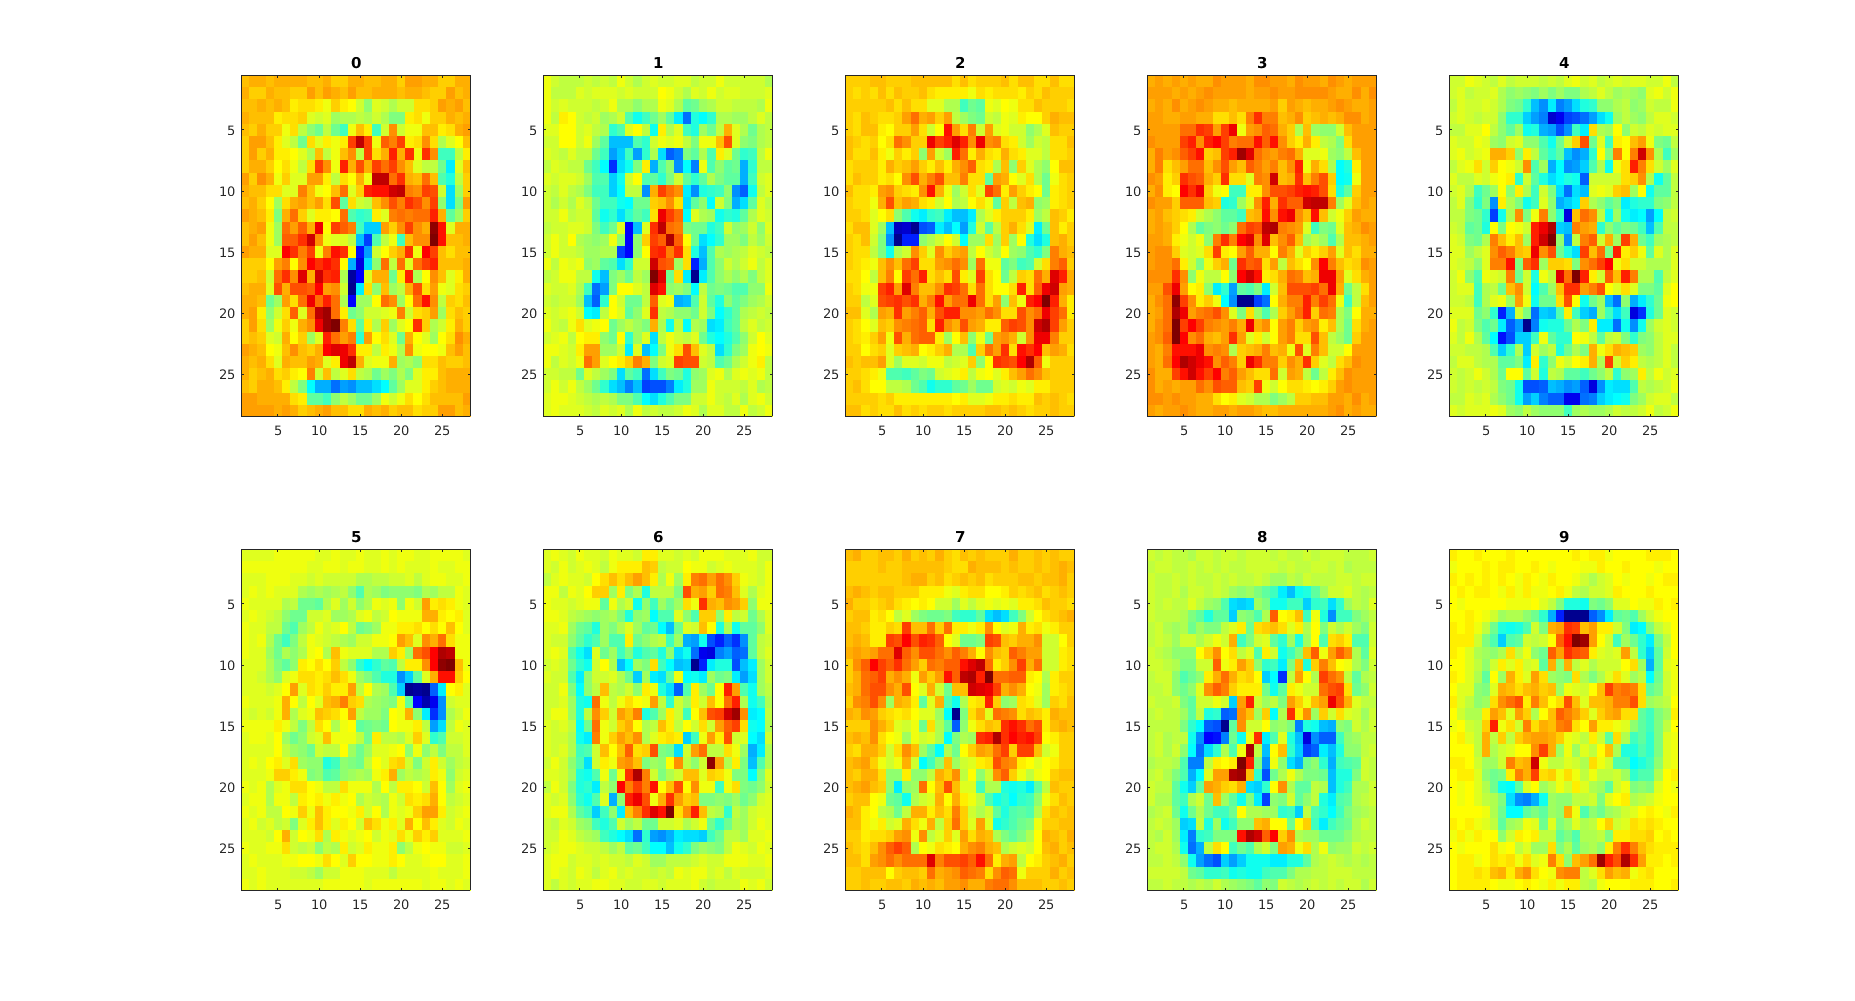
\includegraphics[scale=0.2]{visualize_softmax}
\end{center}
\end{justify}
\end{frame}

\begin{frame}
\frametitle{Autoencoder}
\begin{justify}
\begin{center}
	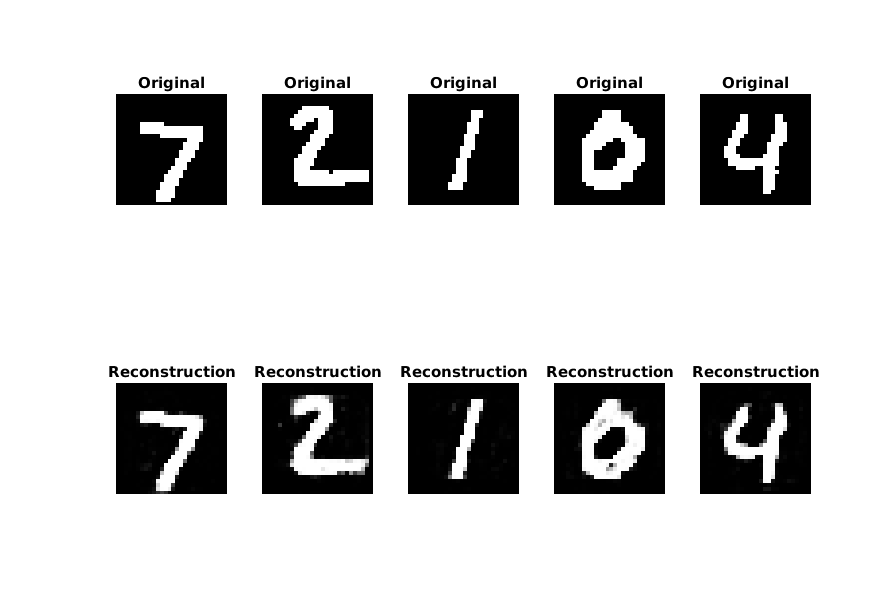
\includegraphics[scale=0.4]{visualize_autoencoder}
\end{center}
\end{justify}
\end{frame}

\section{Low-rank approximation}


\begin{frame}
\frametitle{SVD - Softmax}
\begin{justify}
\begin{center}
	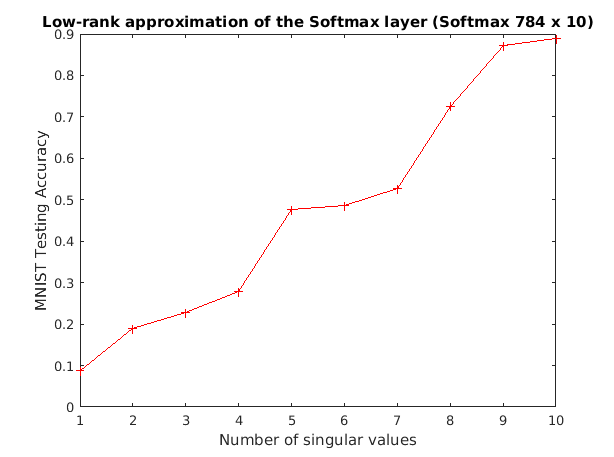
\includegraphics[scale=0.5]{Low-rank-Softmax}
\end{center}
This kind of \textbf{shallow} neural network is \textbf{sensitive} to compression! 
\end{justify}
\end{frame}


\begin{frame}
\frametitle{SVD - Autoencoder}
\begin{justify}
\begin{center}
	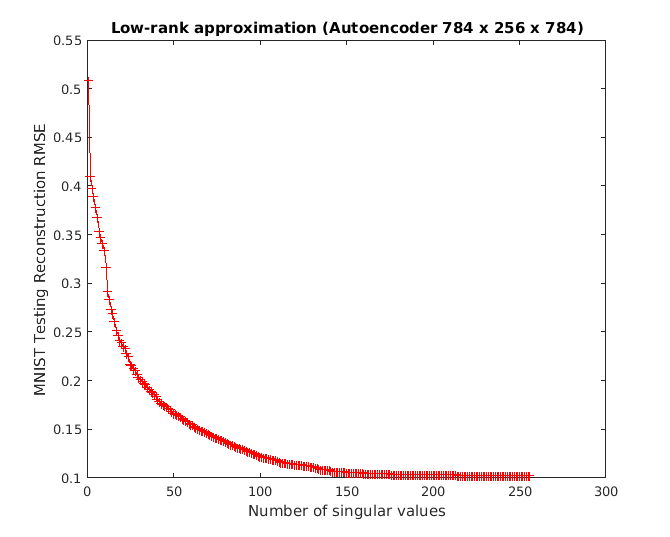
\includegraphics[scale=0.4]{Low-rank-Autoencoder}
\end{center}
We can cut more than half of the number of singular values to get \textbf{acceptable} reconstruction error.
\end{justify}
\end{frame}


\begin{frame}
\frametitle{SVD - MLP}
\begin{justify}
\begin{center}
	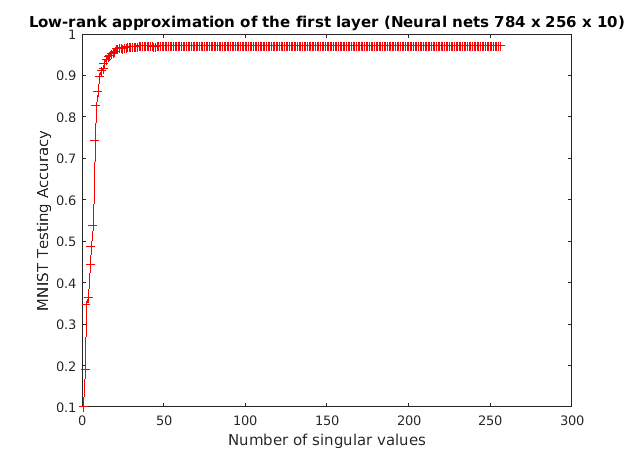
\includegraphics[scale=0.5]{Low-rank-first-layer-Neural-nets}
\end{center}
Only need to keep 18 first singular values to get more than 95\% testing accuracy.
\end{justify}
\end{frame}


\section{Sparsification}


\begin{frame}
\frametitle{Sparsification - Softmax}
\begin{justify}
\begin{center}
	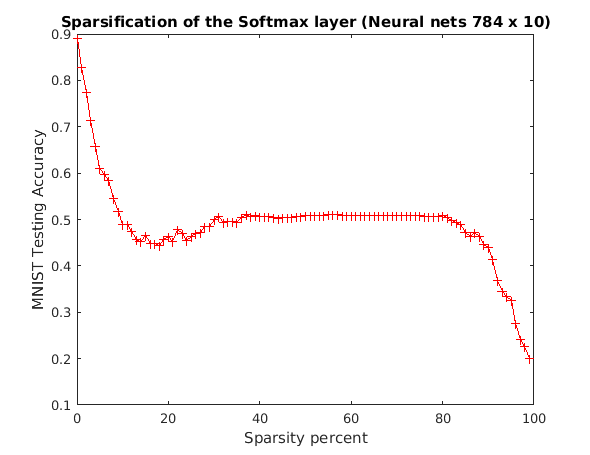
\includegraphics[scale=0.4]{Sparse-Softmax}
\end{center}
Still, \textbf{shallow} nets are \textbf{sensitive} to compression!
\end{justify}
\end{frame}


\begin{frame}
\frametitle{Sparsification - Autoencoder}
\begin{justify}
\begin{center}
	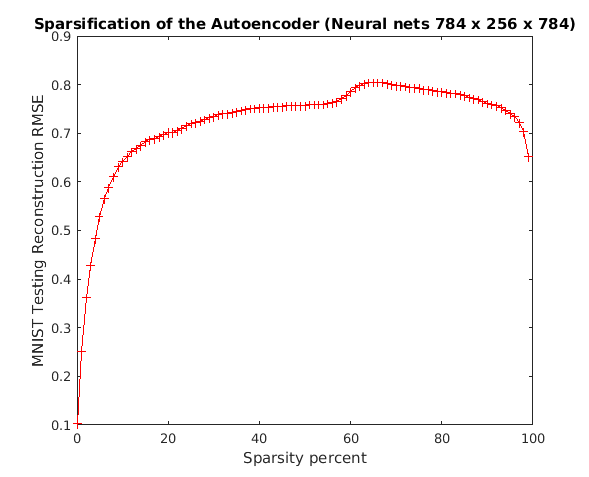
\includegraphics[scale=0.4]{Sparse-Autoencoder}
\end{center}
\end{justify}
Autoencoder is \textbf{sensitive} to \textbf{sparsification}!
\end{frame}


\begin{frame}
\frametitle{Sparsification - MLP}
\begin{justify}
\begin{center}
	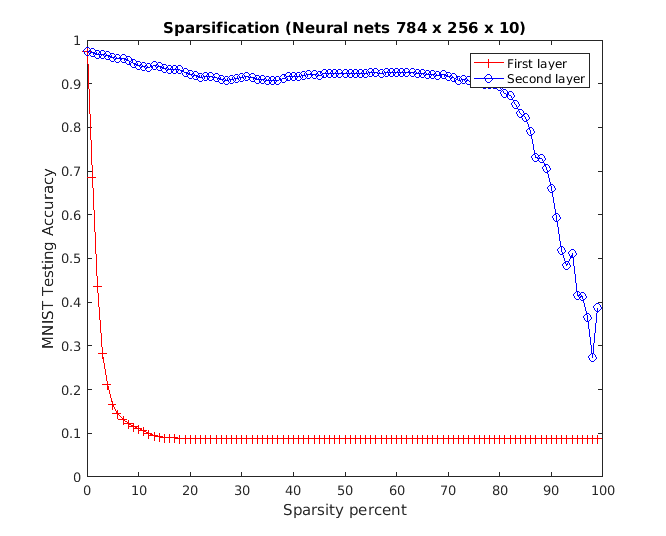
\includegraphics[scale=0.4]{Sparse-Neural-nets}
\end{center}
We can \textbf{throw out} 80\% of the second layer to get more than 90\% testing accuracy. That is \textbf{5}-time compression.
\end{justify}
\end{frame}

\section{K-Means quantization}

\begin{frame}
\frametitle{K-Means - Figure 1}
\begin{justify}
\begin{center}
	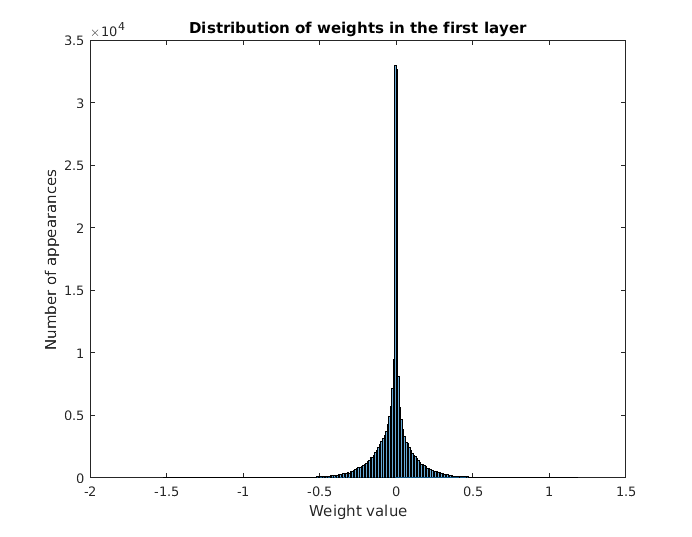
\includegraphics[scale=0.4]{First-layer-Neural-nets-distribution}
\end{center}
\end{justify}
\end{frame}


\begin{frame}
\frametitle{K-Means - Figure 2}
\begin{justify}
\begin{center}
	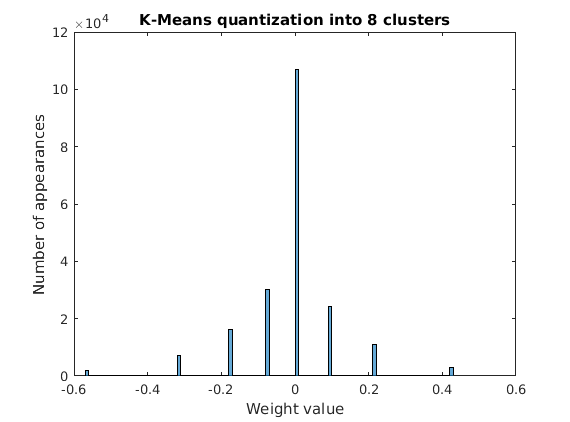
\includegraphics[scale=0.5]{First-layer-Neural-nets-KMeans-8}
\end{center}
\end{justify}
I did the K-Means quantization with a very efficient algorithm $O(k \cdot d \cdot log(n))$ where $k$ is the number of clusters, $d$ is the number of iterations, and $n$ is the number of data points.
\end{frame}


\begin{frame}
\frametitle{K-Means - Figure 3}
\begin{justify}
\begin{center}
	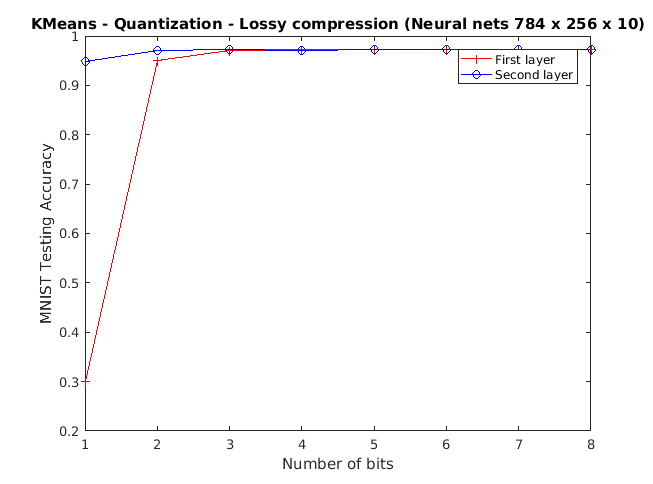
\includegraphics[scale=0.45]{KMeans-quantization-Neural-Nets}
\end{center}
We need only \textbf{2} bits for each weight in the first layer, and \textbf{1} bit for the second layer to get 95\% testing accuracy. Comparing to \textbf{4}-byte double-floating-point, we can obtain \textbf{32} time compression.
\end{justify}
\end{frame}


\section{Fourier Transformation}

\begin{frame}
\frametitle{FFT - Softmax}
\begin{justify}
\begin{center}
	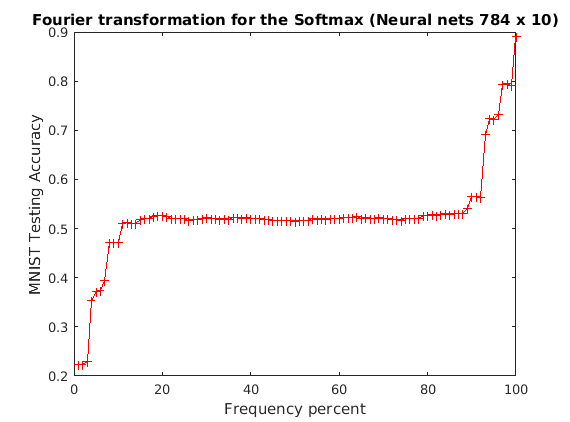
\includegraphics[scale=0.45]{Fourier-Softmax}
\end{center}
Basically, we cannot compress the \textbf{shallow} nets!
\end{justify}
\end{frame}


\begin{frame}
\frametitle{FFT - Autoencoder}
\begin{justify}
\begin{center}
	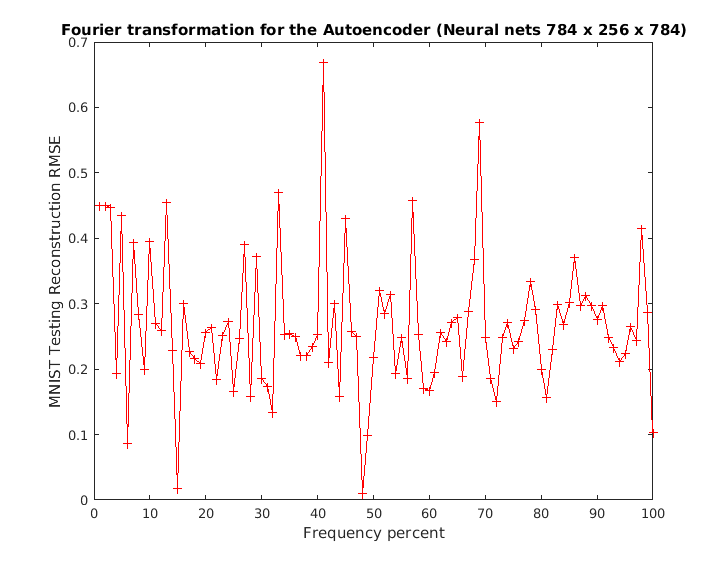
\includegraphics[scale=0.45]{Fourier-Autoencoder}
\end{center}
Autoencoder is \textbf{sensitive} in the \textbf{frequency} domain!
\end{justify}
\end{frame}


\begin{frame}
\frametitle{FFT - MLP}
\begin{justify}
\begin{center}
	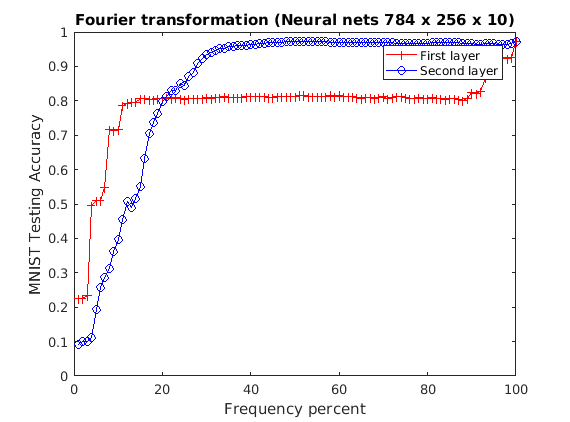
\includegraphics[scale=0.45]{Fourier-Neural-Nets}
\end{center}
\end{justify}
We need to keep \textbf{10\%} of the frequencies in the first layer to get \textbf{80\%} testing accuracy. On the second layer, to obtain \textbf{95\%} accuracy, we need to keep only \textbf{30\%} of the frequencies.
\end{frame}


\section{Conclusions}

\begin{frame}
\frametitle{Conclusions}
\begin{justify}
\begin{itemize}
	\item There are a lot of redundancy in MLP
	\item We only need \textbf{2} bits for each weight in the first layer, and \textbf{1} bits for the second layer
	\item Further lossless compression by Huffman code or LZW can be applicable
\end{itemize}
$$$$
My source code: \\
\href{https://github.com/HyTruongSon/Neural-Nets-Compression}{https://github.com/HyTruongSon/Neural-Nets-Compression}
\end{justify}
\end{frame}


\section{How to compress Deep CNNs?}

\begin{frame}
\frametitle{How to compress Deep CNNs?}
\begin{justify}
Reference:
\begin{itemize}
	\item Multiresolution Matrix Compression/Factorization, Prof. Risi Kondor (UChicago)
	\item Soft Weight-Sharing For Neural Network Compression, ICLR 2017, Karen Ullrich, Max Welling
\end{itemize}
$$$$
Some more practical works:
\begin{itemize}
	\item Compression of Deep Convolutional Neural Networks for Fast and Low Power Mobile Applications, ICLR 2016
	\item Deep Compression: Compressing Deep Neural Networks With Prunning, Trained Quantization and Huffman Coding, ICLR 2016
\end{itemize}
\end{justify}
\end{frame}


\end{sloppypar}
\end{document}

%%%%%%%%%%%%%%%%%%%%%%%%%%
% Template for one frame %
%%%%%%%%%%%%%%%%%%%%%%%%%%

\begin{frame}
\frametitle{}
\begin{itemize}
\end{itemize}
\end{frame}